% Self-Justification Ex Machina
%
% A companion to Sebastian Oberhoff, "Incompleteness Ex Machina" (2018),
% https://www.scottaaronson.com/incompleteness.pdf
%
% Revision 10 (2026-10-26) streamlines revision 9 (commit 93ef87c) without
% changing what is claimed or how it is proved. The main text tells one story,
% for Willard's 2005 system, in Oberhoff's format. The conventions, and the
% proofs that depend on them, are in Appendix A; the 2001 system is in
% Appendix B; the gap in Willard's Theorem 6 and its repair are in Appendix C.
% Willard's results are cited in the text by paper and item only. Their pages
% and proof statuses are in Appendix D, taken from the repository's
% codification (nachlass/codification/registry/results.md). The reading
% notes, the review dispositions and the history of revisions 1-9 are in
% docs/log/2026-10-24-incompleteness-ex-machina-analysis.md.
%
% Build: pdflatex self-justification-ex-machina.tex (twice).

\documentclass[11pt]{article}

\usepackage[T1]{fontenc}
\usepackage{lmodern}
\usepackage[margin=1in]{geometry}
\usepackage{amsmath,amssymb,amsthm}
\usepackage{marvosym}      % \Lightning, Oberhoff's contradiction mark
\usepackage{listings}
\usepackage{booktabs}
\usepackage{array}       % ragged-right p{} columns in the tables
\usepackage{enumitem}
\usepackage{xcolor}
\usepackage{tikz}
\usetikzlibrary{decorations.pathreplacing}  % brace under the figure's number line
\usepackage{microtype}
\usepackage[hidelinks]{hyperref}

% --- Notation -------------------------------------------------------------
\newcommand{\F}{\mathcal{F}}
\newcommand{\Fo}{\mathcal{F}_0}
\newcommand{\G}{\ddot{\mathsf{G}}}          % Oberhoff's computational Goedel sentence
\newcommand{\W}{\ddot{\mathsf{W}}}          % this essay's self-consistency sentence
\newcommand{\Hs}{\mathsf{H}}                % the halting sentence, dual of \G
\newcommand{\Prog}[1]{\mathsf{#1}}
% Formal sentence in Oberhoff's guillemets. In math mode it is boxed with
% \text; in running text it is left unboxed so long sentences can line-break.
\newcommand{\fs}[1]{\ifmmode\text{\guillemotleft#1\guillemotright}\else\guillemotleft#1\guillemotright\fi}
\newcommand{\contra}{~\text{\Lightning}}  % tie: never wrap the mark onto its own line
\newcommand{\Prov}{\mathrm{Prov}}
\newcommand{\Prf}{\mathrm{Prf}}
\newcommand{\Subst}{\mathrm{SUBST}}
\newcommand{\Pair}{\mathrm{Pair}}
\newcommand{\gn}[1]{\ulcorner #1\urcorner}  % Goedel number
\newcommand{\ISD}{\mathrm{IS}_D(A)}
\newcommand{\Mho}{\mho}                     % Willard 2005's bounded Goedel sentence
\newcommand{\sk}{\ensuremath{^\dagger}}    % Willard result without a complete proof
% Oberhoff's case-analysis layout: bold case heads, arrow-led steps.
\newcommand{\Case}[1]{\par\smallskip\noindent\hspace*{1em}\textbf{#1}\par}
\newcommand{\SubCase}[1]{\par\noindent\hspace*{3em}\textbf{#1}\par}
\newlist{steps}{itemize}{2}
\setlist[steps]{label=$\Rightarrow$, leftmargin=5em, itemsep=1pt, topsep=2pt}
\newlist{topsteps}{itemize}{1}
\setlist[topsteps]{label=$\Rightarrow$, leftmargin=3em, itemsep=2pt, topsep=3pt}

\lstset{
  basicstyle=\small\sffamily,
  keywordstyle=\bfseries,
  morekeywords={for,if,else,while,halt},
  columns=fullflexible,
  frame=lines,
  mathescape=true,
  xleftmargin=0pt,
  aboveskip=8pt, belowskip=8pt
}

\theoremstyle{plain}
\newtheorem{theorem}{Theorem}
% Lettered, so this essay's results never collide with Oberhoff's Theorems 1-7
% or with Willard's numbered results, which the text cites by number.
\renewcommand{\thetheorem}{\Alph{theorem}}
\newtheorem{proposition}[theorem]{Proposition}
\newtheorem{lemma}[theorem]{Lemma}
\newtheorem{corollary}[theorem]{Corollary}
\newtheorem{fact}[theorem]{Fact}
\theoremstyle{definition}
\newtheorem*{definition}{Definition}

\title{Self-Justification Ex Machina}
\author{jpt4\thanks{Revision of 26 October 2026, prepared with Claude
  (Anthropic) in the \texttt{sjas} research repository,
  \url{https://github.com/jpt4/sjas}. The pages and proof statuses of
  Willard's results are those recorded in the repository's codification of
  his papers (\texttt{nachlass/codification}); Appendix~\ref{app:sources}
  lists the ones used here.}}
\date{In memory of Dan E. Willard (1948--2023)}

\begin{document}
\maketitle

\begin{abstract}
\noindent
Sebastian Oberhoff's \emph{Incompleteness Ex Machina} proves Gödel's
incompleteness theorems twice, once with sentences and once with programs.
It concludes that the theorems are victory laps, and that the real work was
teaching arithmetic to compute. His proof of the second theorem takes one step
``with some faith''. We argue that this step is a part of Gödel's work in its
own right, and that it has a price. Our witness is Dan Willard's 2005
self-justifying axiom system $\mathrm{IS}_D(A)$, with semantic tableaux or
tableau lists as its deduction method $D$. Every $\Pi_1$ theorem of its base
theory $A$ is true, and $A$ proves every $\Pi_1$ theorem of Peano arithmetic
in Willard's language. The system proves every true $\Sigma_1$ sentence, it
obeys the
first incompleteness theorem, it proves its own consistency, and, by
Willard's theorem, it is consistent. For this system the faith step fails
twice over. In its uniform form it fails because the system cannot prove
that every number can be written down. At the Gödel sentence, built with the
conventions we fix, the step is provably equivalent to the Gödel sentence
itself, and so it is unprovable. Willard's Theorem~6 takes the tableau-list
system over Peano arithmetic in his language and grants it, as an axiom, that
one large enough number exists. The faith returns, and inconsistency comes
with it. The printed proof
of that theorem has a gap, for which we sketch a repair. Gödel's work, viewed
this way, has three parts, not two.
\end{abstract}

\begin{quote}\small
Another way to motivate the axiom system IS is to consider a philosopher's
response to the question of whether multiplication is a function. His first
answer would likely be ``of course yes''. But if one then asked the
philosopher to construct a sequence of natural numbers
$a_0, a_1, a_2, a_3, \ldots$ where $a_0 \ge 2$ and $a_{i+1} = (a_i)^2$, a hedge
would quickly follow because $a_n$ requires at least $2^n$ bits. The expected
response would then be that ``multiplication is a function in theory but not
always in practice''.
\hfill --- Dan Willard, SUNY Albany TR~93-10 (1994)
\end{quote}

% ==========================================================================
\section{One Step On Faith}

Oberhoff's essay~\cite{oberhoff} writes out Gödel's first incompleteness
theorem, Rosser's improvement of it and the second incompleteness theorem as
explicit case analyses. Then it replaces Gödel's sentence $\mathsf{G}$ (``I am
not provable'') by $\G = \fs{$\Prog{P}(\Prog{P})$ doesn't halt}$, where
$\Prog{P}$ is the program
\begin{lstlisting}
P(A) {
  for s $\in$ all possible strings {
    if s is a proof in $\F$ that A(A) doesn't halt {
      halt;
    }
  }
}
\end{lstlisting}
and observes that each case analysis can be copied almost word for word. The
punchline is that $\G$ is $\mathsf{G}$ wearing Clark Kent's glasses:
$\Prog{P}(\Prog{P})$ is searching $\F$'s proofs for a proof of $\G$, so $\G$
says ``I am not provable''. The moral is a refactoring. The hard part of
Gödel's work was teaching arithmetic to compute, which Oberhoff packages as
\begin{quote}
\textbf{Theorem 7} (Turing Completeness of Elementary Arithmetic).
\emph{Every formal system capable of reasoning about elementary arithmetic
can also reason about algorithms,}
\end{quote}
and leaves ``to smarter people''. The incompleteness theorems themselves are
victory laps.

For the first incompleteness theorem we agree completely. This essay is about
one step of the second, the only step that Oberhoff marks as taken on trust:
\begin{quote}
Now we simply observe (with some faith) that there wasn't actually anything
in the reasoning we used to prove this that we couldn't carry out just as
well in $\F$.
\end{quote}
For Peano arithmetic and its relatives the faith is well placed. But some
formal systems reason about algorithms in every sense the first theorem
needs, and for them it is misplaced. Their proofs are cut-free, or reuse
only simple lemmas. They prove their own consistency, and they are
consistent, provided only that their base theory tells no lies about
universal statements. Dan Willard built them, in papers from 1993 to
2020~\cite{w93tr,w01,w05,w06a,w20}. This essay tells their story in
Oberhoff's language. Our headline is that the faith step is not part of the
victory lap. It is a third part of Gödel's work, and it has a price.

\paragraph{Ground rules.} Oberhoff's footnote~2 lets ``$=$'' relate sentences
that are merely logically equivalent, ``provided this is obvious''. We cannot
afford that luxury. Willard's systems are self-justifying for one deduction
method and inconsistent for another, and consistent under one notion of
consistency but not the next. The proofs that tell these cases apart measure
Gödel numbers in bits. A system may prove two sentences equivalent without
proving that one is provable exactly when the other is. So a formal system,
here, is always an axiom system $\F$ together with a deduction method $D$.
Every method we use is \emph{sound and complete}: $\F$ proves $\varphi$ by $D$
exactly when $\varphi$ holds in every model of $\F$. Proof length is what
separates them, and self-justification is a phenomenon of length. Here is the
fact we use most:

\begin{fact}[Closure; Willard 2001, Lemma~7.1B]\label{fact:closure}
If $D$ is sound and complete for $\F$, $\F$ proves $\varphi$ and $\psi$, and
$\varphi \wedge \psi \supset \chi$ holds in every model of $\F$, then $\F$
proves $\chi$.
\end{fact}

\noindent
Everything else is fixed in Appendix~\ref{app:fine}: the languages, the
Gödel numbering, how a negation is put into prenex form, and which sentence
the consistency axiom counts as another's negation. The proofs that depend on
these choices are there too. Every consistency result below, Willard's and
ours, is a theorem of ordinary mathematics under a hypothesis on a base
theory, and none shows a system consistent outright. We cite Willard's
results by year and item, as in ``2005, Theorem~3''. Appendix~\ref{app:sources}
gives their pages and proof statuses. A dagger, as in ``2004,
Theorem~2\sk'', marks a result printed without a complete proof (with a
sketch, a citation, or no proof at all), or one whose printed proof we find
incomplete at our level of detail. Results marked \emph{ours} are proved
here.

% ==========================================================================
\section{Watching And Knowing}
\label{sec:faith}

Here is the first half of Oberhoff's proof that $\G$ is undecidable:

\Case{Suppose $\G$ is provable:}
\SubCase{Or $\neg\G$ isn't provable:}
\begin{steps}
\item Because $\G$ is provable $\Prog{P}(\Prog{P})$ will eventually find such
  a proof after some sequence of steps which we can write out in $\F$.
\item Because this sequence leads to a terminal state this gives a proof of
  $\fs{$\Prog{P}(\Prog{P})$ halts} = \neg\G$.\contra
\end{steps}

\smallskip\noindent
His Theorem~6 asks $\F$ to run this argument on itself. Write $\Prov$ for
provability in $\F$, and $\Hs$ for the $\Sigma_1$ sentence
\fs{$\Prog{P}(\Prog{P})$ halts}, in the form that Appendix~\ref{app:fine}
fixes.\footnote{That form has exactly the proofs of $\neg\G$, and the
consistency axiom counts it as $\G$'s negation. Another $\Sigma_1$ rendering
of \fs{$\Prog{P}(\Prog{P})$ halts} would be a different sentence, with
different proofs.} As statements that $\F$ must prove, the argument has
three steps.
\begin{enumerate}[label=(\arabic*), leftmargin=2.5em]
\item $\Hs \supset \Prov(\gn{\G})$: \fs{if $\Prog{P}(\Prog{P})$ halts, then
  $\G$ is provable}.
\item $\Prov(\gn{\G}) \supset \Prov(\gn{\Hs})$: \fs{if $\G$ is provable, then
  so is \fs{$\Prog{P}(\Prog{P})$ halts}}.
\item $\Prov(\gn{\G}) \wedge \Prov(\gn{\Hs}) \supset \neg\mathit{Con}$:
  \fs{then $\F$ is inconsistent}.
\end{enumerate}
Chaining them gives $\F \vdash \mathit{Con} \supset \G$, which is what
Theorem~6 needs. Step~(1) is the fixed point. $\F$ proves it once it proves
one true bounded sentence and that $\le$ is trichotomous at one number
(Fact~\ref{fact:fp}). Step~(3)
comes free when $\mathit{Con}$ says that no sentence and its negation both
have proofs. If it says only that $0 = 1$ has no proof, step~(3) is a
formalized combination of two proofs into one, and for cut-free deduction
that combination is expensive. Step~(2) is ``$\Prog{P}(\Prog{P})$ will
eventually find such a proof after some sequence of steps which we can write
out in $\F$''. Inside $\F$ it reads: \emph{for every proof $s$ of $\G$ there
is a proof that $\Prog{P}(\Prog{P})$ halts}, namely the one that exhibits $s$
and checks it.

In the first incompleteness theorem, ``which we can write out in $\F$'' was a
fact \emph{about} $\F$, established by us from outside: we are handed a
halting run and we produce the proof. In the second it has to be a theorem
\emph{of} $\F$, about every $s$ at once. The two deserve separate names.

\begin{definition}[Watching]
$\F$ \emph{watches} if it proves every true $\Sigma_1$ sentence.
\end{definition}

\begin{definition}[Knowing that one watches]
$\F$ \emph{knows that it watches} at a sentence $\sigma$ if
$\F \vdash \sigma \supset \Prov(\gn{\sigma})$. It knows that it watches if it
does so at every $\Sigma_1$ sentence.
\end{definition}

\noindent
A program halts exactly when a $\Sigma_1$ sentence about it is true. So
watching is $\Sigma_1$-completeness, and knowing that one watches is its
formalized version, taken one sentence at a time. Section~\ref{sec:transcripts}
adds the uniform version. The third Hilbert--Bernays--Löb derivability
condition~\cite{hb39,lob55}, $\Prov(\gn{\varphi}) \supset
\Prov(\gn{\Prov(\gn{\varphi})})$, is knowing that one watches at the halting
statements of proof searches.

\begin{lemma}[ours]\label{lem:instances}
Let $\F$ watch, with a sound and complete deduction method and a correct
proof predicate.
\begin{enumerate}[label=(\alph*)]
\item $\F$ knows that it watches at every \emph{true} $\Sigma_1$ sentence.
\item If $\F$ proves the fixed point, then step~(2) is $\F$-provably
  equivalent to knowing that it watches at $\Hs$, that is, to
  $\Hs \supset \Prov(\gn{\Hs})$.
\end{enumerate}
\end{lemma}

\begin{proof}
(a) If $\sigma$ is true, $\F$ proves it by watching. So $\Prov(\gn{\sigma})$
is a true $\Sigma_1$ sentence, $\F$ proves that too, and
$\sigma \supset \Prov(\gn{\sigma})$ follows by Fact~\ref{fact:closure}.
(b) $\Hs$ is logically equivalent to $\neg\G$, and the fixed point makes
$\neg\G$ equivalent to $\Prov(\gn{\G})$, so $\F$ proves
$\Hs \leftrightarrow \Prov(\gn{\G})$. The two implications differ only by this
replacement in the antecedent, so $\F$ proves them equivalent
(Fact~\ref{fact:closure}).
\end{proof}

\noindent
So the faith step is not a claim about runs that happen. Those a watching
system sees, and Lemma~\ref{lem:instances}(a) gives it the knowledge for
free. The faith is a claim about a run that does not happen. If $\G$ is
true, then $\Hs$ is false, and step~(2) says that \emph{had}
$\Prog{P}(\Prog{P})$ halted, $\F$ would have seen it.

Every other result in Oberhoff's essay uses at most watching and honesty.
Rosser's version also needs one $\Pi_1$ fact: a run stuck in
\texttt{while true \{\}} stays stuck. As his footnote~12 says, a system that
cannot prove this ``ought to be ashamed of itself''. The classical proof of
the second theorem runs through the derivability conditions. The
computational retelling shows what the third one says.

% ==========================================================================
\section{A Very Stable Genius}
\label{sec:genius}

Oberhoff's moral for the second theorem is ``if you declare yourself a very
stable genius, you're not''. Let us build the genius with his tools. Fix a
base system $\Fo$ with a deduction method, and consider

\noindent\begin{minipage}{\linewidth}
\begin{lstlisting}
C(A) {
  for s $\in$ all possible strings {
    if s is a contradiction in $\Fo + \fs{A(A) doesn't halt}$ {
      halt;
    }
  }
}
\end{lstlisting}
\end{minipage}
where a \emph{contradiction} is either a proof of $0 = 1$ or proofs of a
$\Pi_1$ sentence and of its negation. Willard calls the two corresponding
notions of consistency \emph{Level(0$-$)} and
\emph{Level(1)}.\footnote{We picked $\Prog{C}$ for consistency, and because
it is a circle that never quite closes. Section~\ref{sec:machine} explains
the joke.} Let
\[
\W = \fs{$\Prog{C}(\Prog{C})$ doesn't halt}, \qquad \F = \Fo + \W .
\]
Just as $\G$ says ``I am not provable'', $\W$ says ``$\F$ is consistent''. So
$\F$ proves its own consistency in one line, because the claim is an axiom.

\begin{proposition}[The genius falls; standard]\label{prop:genius}
Let $\Fo$ be a recursively axiomatized extension of $I\Sigma_1$, with
Hilbert-style deduction and the canonical provability predicate. Then, at
either level, $\F = \Fo + \W$ is inconsistent and $\Prog{C}(\Prog{C})$
halts.
\end{proposition}

\begin{proof}
Suppose $\F$ is consistent.
\begin{topsteps}
\item $\F$ proves its own consistency. $\W$ is an axiom, and by the diagonal
  lemma $I\Sigma_1$ proves $\W$ equivalent to $\F$'s consistency. It also
  proves the two levels equivalent: explosion turns a proof of $0=1$ into
  proofs of everything, and modus ponens turns proofs of a sentence and its
  negation into a proof of $0=1$.
\item The derivability conditions hold for $\F$, provably in
  $I\Sigma_1$~\cite{hp93}. In our terms $\F$ knows that it watches, and
  steps (1)--(3) are theorems of $\F$.
\item So Oberhoff's Theorem~6 applies, with its faith step now a theorem, and
  $\F$ cannot prove its own consistency.\contra
\end{topsteps}
So $\F$ is inconsistent. A contradiction in $\F$ is then a finite object, and
$\Prog{C}(\Prog{C})$ finds it.
\end{proof}

Willard records the old verdict on such systems: ``Kleene, Rogers and
Jeroslow [\ldots] each warned their readers that most axiom systems, similar
to $\alpha^*$, were useless on account of their inconsistency, although they
were technically well-defined'' (2005, \S1). Constructing $\W$, he adds, is
``relatively easy, via an application of the Fixed Point Theorem, but this
sentence is ironically typically useless!'' (2016, Example~3.5). To make it
useful, he changed everything else.

% ==========================================================================
\section{Willard's Machine}
\label{sec:machine}

Willard keeps $\Prog{C}$ and $\W$, and changes the language, the deduction
method and the base. We describe his 2005 system $\ISD$. His 2001 system,
which asserts only Level(0$-$) consistency, is in Appendix~\ref{app:2001}.

\paragraph{The language.} There are constants for $0$ and $1$, two growth
functions, $+$ and $\mathit{Double}(x) = x + x$, and six functions that
never exceed their largest argument: truncated subtraction, division, roots,
maximum, logarithm and a bit count. Every number $n \ge 2$ has a name
$\bar n$ with at most $2\log_2 n$ growth symbols, which is its binary
notation. Multiplication is not a function symbol. Its graph is a bounded
formula, so the system knows the laws of multiplication but not that every
product exists. ``Bounded'', ``$\Pi_1$'' and ``$\Sigma_1$'' mean what they
usually mean, for these function symbols. Peano arithmetic in this language
is called $\mathrm{PA}{+}$.

\paragraph{The axioms.} $A$ is any axiom system in this language with a
bounded proof predicate, and $D$ is a deduction method. The axioms of $\ISD$
fall into four groups (2005, \S3).
\begin{itemize}[leftmargin=1.5em]
\item \textbf{Group-0} (names) defines $0$, $1$, $+$ and $\mathit{Double}$.
\item \textbf{Group-1} (watching) is a finite set of true $\Pi_1$ sentences
  that proves every true bounded sentence.
\item \textbf{Group-2} (inheritance) is
  $\forall p\,[\Prf_A(\gn{\Phi}, p) \supset \Phi]$, for every $\Pi_1$ sentence
  $\Phi$. Whatever $\Pi_1$ sentence $A$ proves, $\ISD$ proves too.
\item \textbf{Group-3} (self-reference) is $\W$ at Level(1): no $\Pi_1$
  sentence and its negation both have $D$-proofs from $\ISD$. It is built by
  the same fixed point as $\G$ (Appendix~\ref{app:fine}).
\end{itemize}

\paragraph{The deduction methods.} A \emph{semantic tableau} proof of $\Phi$
is a tree whose root is $\neg\Phi$ in prenex form. It grows by elimination
rules alone, with no cut, and every branch closes with some sentence and its
negation. A \emph{tableau list} is a list of tableau proofs, each of which may
use the earlier conclusions as axioms, all of them $\Pi_1$ or $\Sigma_1$. This
is modus ponens restricted to lemmas with one unbounded quantifier block.

\begin{theorem}[Willard 2005, Theorems 3 and 5]\label{thm:willard}
If every $\Pi_1$ theorem of $A$ is true, then $\ISD$ is consistent, both for
semantic tableaux and for tableau lists. With the conventions of
Appendix~\ref{app:fine}, its Group-3 axiom is in fact true.
\end{theorem}

\noindent
With Hilbert-style deduction the same construction ``will be automatically
inconsistent'', by theorems of Pudlák and Solovay (2005, \S3) that
Section~\ref{sec:price} returns to. Meanwhile $\ISD$ reasons about algorithms
perfectly well.

\begin{lemma}[ours]\label{lem:watch}
For either deduction method, $\ISD$ watches. If every $\Pi_1$ theorem of $A$
is true, then every theorem of $\ISD$ is true, and the proof predicate that
its Group-3 axiom uses, Willard's $\mathit{SubstPrf}(\bar n_3, \cdot, \cdot)$
(Appendix~\ref{app:fine}), is a correct bounded proof predicate for $\ISD$.
\end{lemma}

\begin{proof}
A true $\Sigma_1$ sentence $\exists\vec x\,\delta(\vec x)$ with witnesses
$\vec k$ follows by logic from the true bounded sentence
$\delta(\bar{\vec k})$, which Groups 0 and 1 prove, and
Fact~\ref{fact:closure} does the rest. Truth and correctness are proved in
Appendix~\ref{app:fine}.
\end{proof}

\noindent
Suppose, then, that every $\Pi_1$ theorem of $A$ is true and that $A$ proves
every $\Pi_1$ theorem of $\mathrm{PA}{+}$. Then $\ISD$ obeys the first
incompleteness theorem, in Rosser's form as well. $\G$ is unprovable by
Corollary~\ref{cor:isd}, $\neg\G$ is false and so unprovable, and Rosser's
loop fact is inherited from $\mathrm{PA}{+}$ through Group-2
(Appendix~\ref{app:fine}). In 1994 Willard described his first system in
these terms, as ``a class of structures, lying halfway between Peano
Arithmetic and Presburger Arithmetic, which satisfy Godel's First but not
Second Incompleteness Theorem'' (TR 93-10).

\subsection*{Why the genius survives}

Willard's 2005 consistency proof rests on one idea, \emph{horizons}. Call a
universal sentence $\forall\vec x\,\psi$ \emph{true up to} $a$ if $\psi$
holds whenever every $x_i \le a$. Call an existential sentence
$\exists\vec x\,\psi$ \emph{witnessed below} $b$ if some $\vec x \le b$
satisfies $\psi$. Bounded quantifiers inside $\psi$ are left alone. For
$a > b \ge 1$, a system is \emph{Normed}$(a,b)$ if each axiom is a universal
sentence true up to $a$ or an existential sentence witnessed below $b$
(Definition~4). A deduction method is \emph{$\theta$-compactified} if proofs
cannot see much past their axioms. Suppose $p \le \lceil a/b\rceil + 1$ is a
proof of $\Phi$ from a Normed$(a,b)$ system. Then an existential $\Phi$ must be
witnessed below $b\,p^\theta$, and a universal $\Phi$ must be true up to
$a/p^\theta$ (Definition~5). Tableaux and tableau lists are
$\tfrac14$-compactified (Theorems~2 and~4). Here is Theorem~1 with
$\theta = \tfrac14$ (Figure~\ref{fig:horizon}).

\Case{Suppose $\ISD$ is inconsistent:}
\begin{steps}
\item Then $\Prog{C}(\Prog{C})$ halts. There are proofs $j_1$ of a $\Pi_1$
  sentence $\Phi$ and $j_2$ of its negation, and by Appendix~\ref{app:fine}
  $j_2$ also proves the $\Sigma_1$ sentence $\Psi$ that negates $\Phi$.
  Choose such a pair with $m = \max(j_1, j_2)$ as small as possible.
\item Groups 0--2 are true. Group-3 is false, but its least counterexample is
  this pair, so it is true up to $m - 1$. Hence $\ISD$ is
  Normed$(m-1, 1)$.
\item So $j_1$ certifies $\Phi$ true up to $(m-1)/m^{1/4}$, and $j_2$ finds a
  witness for $\Psi$ below $m^{1/4}$.
\item But $(m-1)/m^{1/4} > m^{1/4}$, so the witness for $\Psi$ lies where
  $\Phi$ has been certified.\footnote{The inequality needs $m \ge 3$. Every
  proof's Gödel number is far larger, since it is at least $32 \cdot
  64^2$.}\contra
\end{steps}

\noindent
The work is in the third arrow, and it is a program. Suppose a tableau $p$
proves an existential sentence $\Phi$ from a Normed$(a,b)$ system, but $\Phi$
has no witness below $b\,p^{1/4}$. Then the root $\neg\Phi$ is a universal
sentence true up to $b\,p^{1/4}$, so the axioms together with the root form a
Normed$(b\,p^{1/4}, b)$ system. Now walk down the tree (Lemma~1):

\noindent\begin{minipage}{\linewidth}
\begin{lstlisting}
Probe(p) {
  N := the root of p;
  while N is not a leaf {
    if N has two children {
      N := its left child if that is true, else its right child;
    } else {
      N := its only child;
      if N introduces a parameter u {
        give u the least value that keeps the branch positive;
      }
    }
  }
}
\end{lstlisting}
\end{minipage}
Here a node is \emph{true} if its sentence holds under the values given so
far, read with the horizons: universals up to $b\,p^{1/4}$, existentials below
$b$, bounded sentences outright (Willard's condition~II). The branch is
\emph{positive} if its nodes are true and each parameter has a value at most
$b \cdot 2^\Delta$, where $\Delta$ counts the function symbols on the branch
down to the node that introduced it (Eq.~19). Each function symbol at most
doubles a value. So, by a nine-case induction, with one case for axioms and
one for each of the eight elimination rules, the walk never gets stuck while
every branch carries fewer than
$\log_2(b\,p^{1/4}) - \log_2 b = \tfrac14 \log_2 p$ function symbols
(Lemma~1). Willard's encoding spends more than five bits on each one, so a
branch carries fewer than $\tfrac15\log_2 p$ (Eq.~20).\footnote{Larger Gödel numbers only widen
the margin. Willard notes that his theorems ``would also be valid for
uncompressed encoding methods'' (2005, Appendix~A). What would break this
proof is a notation more compact than it allows, with four bits or fewer per
function symbol along the deepest branch.} The branch it finds cannot close,
because a closing pair would be two bounded sentences that are both true
(Lemma~2). So $p$ has an open branch, and it is not a proof.\contra{}
Universal sentences are handled by permuting the quantifiers (2005,
Appendix~B). Theorem~3 follows, and Theorem~5 follows in the same way from
Theorem~4.

\begin{figure}[tb]
\centering
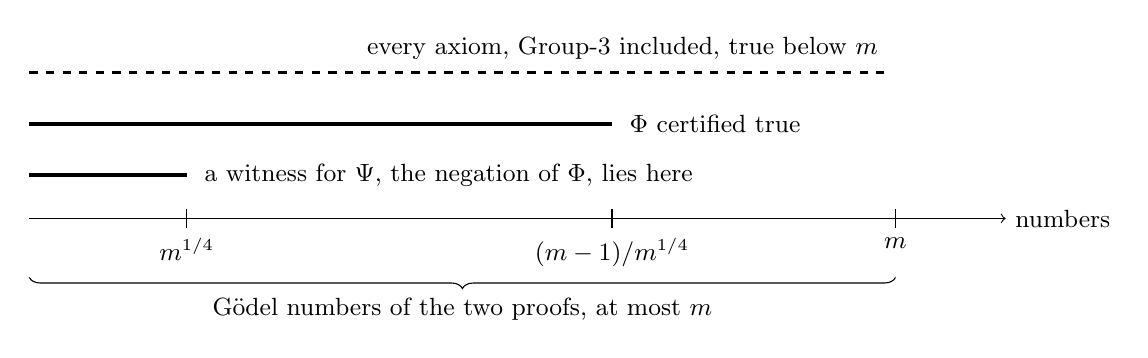
\begin{tikzpicture}[x=1cm,y=1cm,font=\small]
  \draw[->] (0,0) -- (12.4,0) node[right] {numbers};
  \foreach \x/\l in {2.0/{$m^{1/4}$}, 7.4/{$(m-1)/m^{1/4}$}, 11.0/{$m$}}
    { \draw (\x,0.12) -- (\x,-0.12) node[below] {\l}; }
  \draw[very thick] (0,0.55) -- (2.0,0.55);
  \node[anchor=west] at (2.1,0.55) {a witness for $\Psi$, the negation of $\Phi$, lies here};
  \draw[very thick] (0,1.2) -- (7.4,1.2);
  \node[anchor=west] at (7.5,1.2) {$\Phi$ certified true};
  \draw[very thick, dashed] (0,1.85) -- (10.9,1.85);
  \node[anchor=south east] at (10.9,1.9) {every axiom, Group-3 included, true below $m$};
  \draw[decorate,decoration={brace,amplitude=4pt,mirror}] (0,-0.75) -- (11.0,-0.75)
    node[midway,below=4pt] {Gödel numbers of the two proofs, at most $m$};
\end{tikzpicture}
\caption{The two horizons in Willard's proof (schematic, not to scale). A
universal theorem is certified out to its horizon, and an existential one
finds its witness inside its horizon. When the horizons are short compared
with the proofs, the two collide in the region where every axiom is true.}
\label{fig:horizon}
\end{figure}

$\Prog{Probe}$ takes any purported refutation of the system and returns an
open branch, with values for its parameters. Willard's consistency proof is
therefore a machine that defeats each refutation by running it, in a universe
barely larger than the refutation itself. That is self-justification ex
machina in the most literal sense. It is also the joke in the name
$\Prog{C}$. The searcher hunts for a tree all of whose branches close, and the
walk always finds one that stays open. $\ISD$ does not prove that the machine
works. That part is external, and the system has only the axiom.

% ==========================================================================
\section{Transcripts Are Bigger Than Runs}
\label{sec:transcripts}

Why should knowing be harder than watching? The natural proof of step~(2)
takes a proof $s$ of $\G$ and produces the proof $t$ of
\fs{$\Prog{P}(\Prog{P})$ halts} that exhibits $s$ and checks it. In a
language whose only growth functions are $+$ and $\mathit{Double}$,
exhibiting $s$ costs a term, and terms are expensive.

\begin{lemma}[ours]\label{lem:transcript}
In Willard's 2005 language and encoding, every tableau proof that contains a
closed term of value $v \ge 2$ has a Gödel number greater than $v^5$.
\end{lemma}

\begin{proof}
A closed term with $L$ function symbols has value at most $2^L$, because $+$
and $\mathit{Double}$ at most double their largest argument and the other
functions do not increase it. So a term of value $v$ has at least $\log_2 v$
function symbols, and every branch through the node that contains it
carries at least that many. Willard's encoding guarantees that every branch
of a proof $p$ carries fewer than $\tfrac15 \log_2 p$ function symbols
(Eq.~20). Hence $\log_2 p > 5 \log_2 v$.
\end{proof}

\noindent
So the transcript $t$ is bigger than the fifth power of the run $s$ it
records. The natural proof of step~(2) asks $\F$ to believe that
$s \mapsto t$ is defined everywhere. Willard's systems cannot believe that of
any function that outgrows every linear one. The reason lies in how a proof
from universal axioms produces the numbers it claims exist.

\begin{proposition}[Linear witnesses; ours]\label{prop:herbrand}
Let $\F$ be a set of true sentences of Willard's 2005 language, each bounded
or $\Pi_1$, and let $\delta(\vec x, \vec y)$ be bounded. If $\F$ proves
$\forall\vec x\,\exists\vec y\,\delta(\vec x, \vec y)$ by any sound
deduction method, then there is a number $k$ such that every $\vec x$ has a
witness $\vec y \le k\,(x_1 + \cdots + x_m + 1)$.
\end{proposition}

\noindent
The proof, by compactness and an initial segment closed under the function
symbols, is in Appendix~\ref{app:fine}. For intuition, Herbrand's theorem
would present the witnesses as terms in $\vec x$. A term of depth $d$ built
from $+$, $\mathit{Double}$ and the non-growth functions is at most $2^d$
times its largest argument. So $k$ is like $2^d$. That is exponential in the
size of the proof, but it is fixed once the proof is, while $\vec x$ ranges
over all numbers. With multiplication, a term of depth $d$ can grow like
$x^{2^d}$. That is the whole difference.

Write $\mathrm{Num}(x,y)$ for a bounded formula saying that $y$ is the Gödel
number of the sentence $\bar x = \bar x$. For a bounded formula $\delta(x)$,
let $\mathrm{Num}_\delta(x,y)$ say that $y$ codes $\delta(\bar x)$. Say that
$\F$ \emph{knows uniformly that it watches} $\delta$ if
\[
\F \vdash \forall x\,[\delta(x) \supset \exists y\,\exists
q\,(\mathrm{Num}_\delta(x,y) \wedge \Prf(y,q))].
\]
This is $\Sigma_1$-completeness formalized with a free variable. Recursively
axiomatized extensions of $I\Sigma_1$ prove it for their canonical
provability predicate, and they derive the third derivability condition from
it~\cite{hp93}. Willard's systems do not.

\begin{corollary}[ours]\label{cor:uniform}
Suppose every $\Pi_1$ theorem of $A$ is true. Then $\ISD$ proves neither
$\forall x\,\exists y\; y = x \cdot x$ nor
$\forall x\,\exists y\,\mathrm{Num}(x,y)$. It cannot prove that every number
has a written name, so it does not know uniformly that it watches even the
formula $x = x$. The deduction method matters only through the truth of the
axioms, so no sound method proves these sentences from them.
\end{corollary}

\begin{proof}
Every axiom of $\ISD$ is true and is bounded or $\Pi_1$. For Groups 0--2 this
follows from the hypothesis and Willard's remark that they ``can be encoded
as $\Pi_1^*$ sentences'' (2005, \S5). For Group-3 it is
Theorem~\ref{thm:willard}. So Proposition~\ref{prop:herbrand} applies, and
only linear witnesses are available. But $x^2$ exceeds $k(x+1)$ once $x > 2k$.
And the code of $\bar x = \bar x$ is at least $x^6/2$: the term $\bar x$ has
at least $\log_2 x$ function symbols, one byte each, so the code is at least
$32 \cdot 64^{\log_2 x - 1}$ (Appendix~\ref{app:fine}). Finally, knowing
uniformly that it watches $x = x$ implies $\forall x\,\exists
y\,\mathrm{Num}(x,y)$.
\end{proof}

\noindent
Willard saw this in 1994 (TR 93-10):
\begin{quote}\small
This means there will always be adequate memory for writing $b_n$'s binary
encoding when there is sufficient memory for storing a semantic tableaux
proof of its existence (whereas the same is plainly not true \emph{when
multiplication is assumed to be a function}). For instance, multiplication
allows one to establish the existence of a number $a_{300}$ (in a proof with
approximately 300 lines), whose binary encoding requires \emph{more digits}
than the number of atoms in the universe.
\end{quote}
Here $b_{i+1} = b_i + b_i$ and $a_{i+1} = (a_i)^2$. A proof of $n$ doublings
names a number of about $n$ bits, and a proof of $n$ squarings names one of
about $2^n$ bits. Later he put it as a comparison between a proof's Gödel
number and the integer the proof shows to exist. Under additive naming the
proof is always the bigger of the two, and under multiplicative naming it can
be far smaller (2006a, Remark~3).

The faith step in Oberhoff's proof is a single closed sentence about the
Gödel sentence, though, and there the totality claim is vacuous. If $\G$ is
true, no proof of $\G$ exists, so ``for every $s$ there is a transcript''
holds trivially. Proposition~\ref{prop:herbrand} cannot catch step~(2)
failing, so something else must.

% ==========================================================================
\section{Taking Off The Glasses}
\label{sec:backwards}

Oberhoff's \S5 takes the glasses off $\G$ and finds ``I am not provable''
underneath. Let us take them off the faith step. One might think that
Willard's system is self-justifying merely because nobody has managed to
prove step~(2) in it. In fact it cannot prove it, and the reason is
Oberhoff's Theorem~6 run backwards.

\begin{proposition}[ours]\label{prop:backwards}
Let $\F$ have a sound and complete deduction method and a correct bounded
proof predicate, and build $\G$ and $\Hs$ from them as in
Appendix~\ref{app:fine}. Suppose:
\begin{enumerate}[label=(H\arabic*), leftmargin=3em]
\item $\F$ is Level(0$-$) consistent;
\item $\F$ watches;
\item $\F$ proves the true bounded sentences, and that $\le$ is trichotomous at
  $\gn{\G}$;
\item $\F$ proves its own Level(1) consistency, for a bounded pairing of
  sentences with their negations that pairs $\G$ with $\Hs$.
\end{enumerate}
Then $\F$ proves that step~(2) is equivalent to $\G$, and so is knowing that
it watches at $\Hs$. Yet $\F$ does not prove $\G$. So $\F$ proves neither
step~(2) nor $\Hs \supset \Prov(\gn{\Hs})$, although both are true. That $\F$
does not prove $\G$ uses only (H1), (H2), the soundness and completeness of
the method, the correctness of the proof predicate, and the half of the fixed
point that follows from one true bounded sentence ((FP$\Rightarrow$) of
Fact~\ref{fact:fp}).
\end{proposition}

\begin{proof}
First, $\F$ proves step~(3). By (H3) it proves that the pairing pairs $\G$
with $\Hs$, and by (H4) two paired sentences never both have proofs. By (H3)
and Fact~\ref{fact:fp}, $\F$ also proves the fixed point
$\G \leftrightarrow \neg\Prov(\gn{\G})$. Now argue inside $\F$.

\Case{Suppose step (2):}
\begin{steps}
\item If $\G$ had a proof, then so would $\Hs$, by step~(2), and step~(3)
  forbids that.
\item So $\neg\Prov(\gn{\G})$, which by the fixed point is $\G$.
\end{steps}
\Case{Suppose $\G$:}
\begin{steps}
\item By the fixed point, $\G$ has no proof. So step~(2), whose antecedent is
  $\Prov(\gn{\G})$, holds vacuously.
\end{steps}

\smallskip\noindent
Both arguments use only theorems of $\F$ and logic, so
Fact~\ref{fact:closure} turns them into a proof in $\F$ that step~(2) is
equivalent to $\G$. Lemma~\ref{lem:instances}(b) does the same for
$\Hs \supset \Prov(\gn{\Hs})$. That $\F$ does not prove $\G$ is Oberhoff's
\S4, case~1.

\Case{Suppose $\F$ proves $\G$:}
\begin{steps}
\item The proof predicate is correct, so $\Prov(\gn{\G})$ is a true $\Sigma_1$
  sentence, and $\F$ proves it by watching. $\F$ sees $\Prog{P}(\Prog{P})$
  halt.
\item By (FP$\Rightarrow$), $\F$ proves $\neg\G$ as well, and hence $0 = 1$
  (Fact~\ref{fact:closure}), against (H1).\contra
\end{steps}

\smallskip\noindent
Finally, $\G$ has no proof and the proof predicate is correct, so $\G$ is
true. Step~(2) is true because its antecedent is false, and
$\Hs \supset \Prov(\gn{\Hs})$ is true because $\Hs$ is false.
\end{proof}

\noindent
So the faith step is the Gödel sentence wearing glasses. The two are provably
equivalent, and they are true and unprovable for the same reason. The step
fails at the $\Sigma_1$ sentence that says $\Prog{P}(\Prog{P})$ halts, and at
every sentence with the same proofs.\footnote{A $\Sigma_1$ rendering of
\fs{$\Prog{P}(\Prog{P})$ halts} with \emph{different} proofs, such as
$\exists x\,\exists h\,[\Subst(\bar n, h) \wedge \Prf(h, x)]$ in the notation
of Appendix~\ref{app:fine}, is a different sentence, because provability is
sensitive to codes. The proposition says nothing about it.} Willard's system
meets every hypothesis.

\begin{corollary}[ours]\label{cor:isd}
Let $A$ prove every $\Pi_1$ theorem of $\mathrm{PA}{+}$, let every $\Pi_1$
theorem of $A$ be true, and build $\G$ and $\Hs$ from Willard's own proof
predicate for $\ISD$, with the conventions of Appendix~\ref{app:fine}. Then,
for semantic tableaux and for tableau lists, $\ISD$ proves neither $\G$, nor
step~(2), nor $\Hs \supset \Prov(\gn{\Hs})$.
\end{corollary}

\begin{proof}
(H1) follows from Theorem~\ref{thm:willard}, and (H2) is
Lemma~\ref{lem:watch}. For (H3), Groups 0 and 1 prove the true bounded
sentences. Trichotomy is a $\Pi_1$ theorem of $\mathrm{PA}{+}$, so $A$ proves
it, and Group-2 hands it down. (H4) is the Group-3 axiom itself. The proof
predicate is correct by Lemma~\ref{lem:watch}. Appendix~\ref{app:fine} gives
the details.
\end{proof}

The proposition is a contrapositive and claims no new method. Its sibling in
Willard is 2001, Theorem~7.2: by the same fixed point, no consistent system of
this kind proves canonical reflection for all its $\Pi_1$ sentences. In 1994
Willard had already set out the alternatives: ``every axiom system either
fails to prove its consistency or fails to meet the full Hilbert-Bernays
conditions'' (TR 93-10). The computational reading adds \emph{which}
condition fails, at \emph{which} sentence, and that the failing instance is
the Gödel sentence in disguise. What Willard adds, and no contrapositive can
supply, is that systems on the far side of the alternative \emph{exist}.

% ==========================================================================
\section{The Price Of Faith}
\label{sec:price}

If withholding faith is what lets $\W$ survive, the second theorem should
return as soon as the system can afford the transcripts. Willard spent the
second half of his career proving that it does.

\subsection*{One big number}

Willard's 2005 paper ends with the experiment. Let $2^m_k$ be the least $z$
whose $k$-fold base-2 logarithm is at least $m$, roughly a tower of $k$
exponentials topped by $m$. Let $\Upsilon(k,m)$ be the true $\Sigma_1$
sentence ``a number at least $2^m_k$ exists''. $\mathrm{NS}^{k,m}_D(A)$ is
$\ISD$ with $\Upsilon(k,m)$ added to Group-0, and with Group-3 adjusted to the
larger system (Definitions~2 and~3). Both systems prove $\Upsilon(k,m)$, but
only one has it for free.

Let $\Mho$ be the bounded Gödel sentence ``I have no short proof'', that is,
no proof $p$ with $\mathrm{Log}^{k-1}(p) < m$ (Eq.~24). Lemma~4 is the faith
step, bounded. For large $k$, Peano arithmetic in this language,
$\mathrm{PA}{+}$, proves a $\Pi_1$ sentence whose instance in Willard's proof
is (27). It says that for every short proof $p$ of $\Mho$ and every $n$ with
$\mathrm{Log}^k(n) \ge m$ there is a transcript $q < n$ that checks $p$ and
proves ``$\Mho$ is provable''.
Lemma~4 rests on Lemma~3\sk, a sketch showing that checking a proof is
cheap. Because the transcript is bounded by $n$, (27) is $\Pi_1$, and the
system inherits it through Group-2. What is missing is $n$, and
$\Upsilon(k,m)$ supplies it.

\begin{theorem}[Willard 2005, Theorem~6\sk]\label{thm:ns}
For tableau lists there is a $k_0$ such that, for every $k > k_0$,
$\mathrm{NS}^{k,m}_D(\mathrm{PA}{+})$ is inconsistent.
\end{theorem}

\noindent
Willard's proof is a tableau list $W$ of seven steps, and it is Oberhoff's
Theorem~6 with the faith supplied:
\begin{topsteps}
\item (27), inherited from $\mathrm{PA}{+}$: the faith step, below $n$.
\item The Group-3 axiom, at $\Mho$ and its negation: step~(3).
\item So no transcript exists: no $p$ and $q$ satisfy
  $\mathit{CheckProof}(\gn{\Mho}, p, q)$. As printed, this step does not
  follow from the one before; see below.
\item With (27), no short proof of $\Mho$ coexists with a number $n$ that
  large. $\Upsilon(k,m)$, an axiom, supplies $n$, so no short proof of $\Mho$
  exists. That is $\Mho$ itself.
\item Because $\Upsilon(k,m)$ cost nothing, $W$ is short. For $k > k_0$ its
  Gödel number is below $2^m_{k-1}$, so $W$ is one of the short proofs that
  $\Mho$ says do not exist. Watching $W$, the system proves that such a proof
  exists, and so it refutes $\Mho$.\contra
\end{topsteps}

\noindent
The dagger is ours. At our level of detail, the third arrow needs the
transcript to prove the sentence that the consistency axiom pairs with
$\Mho$. As printed, it proves a different one.
Appendix~\ref{app:ns} sketches a repair, so we count the theorem as a sketch,
although Willard prints a full proof. He also states, without proof,
versions for semantic tableaux and other cut-free methods, for an empty base
theory, and without the axioms that make addition and doubling total
(Remark~8\sk).

Why does the argument not run in $\mathrm{IS}_D(\mathrm{PA}{+})$, which
proves $\Upsilon(k,m)$ too? Willard's own engine answers; the observation is
ours. Assume, as Theorem~\ref{thm:willard} does with $A = \mathrm{PA}{+}$,
that every $\Pi_1$ theorem of $\mathrm{PA}{+}$ is true. Then every axiom of
$\mathrm{IS}_D(\mathrm{PA}{+})$ is a true $\Pi_1$ sentence. Groups 0--2 ``can
be encoded as $\Pi_1^*$ sentences'' (2005, \S5), and Group-3 is true by
Theorem~\ref{thm:willard}. So the system is Normed$(a, 1)$ for every
$a > 1$. Let $p > 1$ be a proof of $\Upsilon(k,m)$, and take $a = p$, so
that $p \le \lceil a/1 \rceil + 1$. Then $\tfrac14$-compactification puts a
witness for $\Upsilon(k,m)$ at or below $p^{1/4}$. The least witness is
$2^m_k$, so $p \ge (2^m_k)^4$. In a list that uses $\Upsilon(k,m)$ as a
lemma, the components up to the lemma form a list proof of it, and their
bytes begin the whole list. So the whole list's Gödel number is at least
$(2^m_k)^4$ too. That is far beyond the short proofs that $\Mho$ speaks of.
In Willard's words, ``a
Kleene-like Group-3 axiom has a different connotation when it refers to a
short proof, referencing itself, than when it refers to a long such proof''
(2005, \S6). The asymmetry is exact. Adding a true $\Pi_1$ sentence instead
of $\Upsilon(k,m)$ preserves consistency (2005, \S6\sk). A universal axiom
constrains. An existential axiom supplies a number, and the number is what
the faith step was missing.

\subsection*{Squaring}

Give a tableau system multiplication as a total function, and a proof of $n$
lines can name $2^{2^n}$, by $u_0 = 2$ and $u_{i+1} = u_i \cdot u_i$.
Transcripts become affordable, and the second theorem returns. Willard
located the mechanism himself (2000, \S5):
\begin{quote}\small
Many readers will smile with amusement when they learn the true reason that
the Semantic Tableaux version of the Second Incompleteness Theorem breaks
down when Multiplication is changed from a total function into a 3-way
relation. It is essentially that Lemma 8 and its short proof then become no
longer valid. \ldots{} Without it, our proof of the Semantic Tableaux version
of the Second Incompleteness Theorem collapses entirely!
\end{quote}
His Lemma~8 is the squaring construction: a short tableau proof that a
number about as large as $z$ exists. With it, the second theorem holds for
semantic tableaux at Level(0$-$). It holds for consistent finite extensions
of $Q + V$, for an explicit $\Pi_1$ sentence $V$ (2002a, Theorem~3.5;
Theorem~3.4 shows that $Q + V$ is consistent). It also holds for every consistent extension of $I\Sigma_0$ in
either of its two standard axiomatizations (2007, Theorem~6). That answers a
question Paris and Wilkie asked in 1981. On the positive side,
$\theta$-compactification becomes ``impossible to satisfy'' once
multiplication is a function symbol (2005, Remark~4\sk).

\subsection*{Subroutines}

A Hilbert-style proof can prove a lemma once and use it many times, so modus
ponens is a subroutine call. A tableau must inline every use, and inlining can
be astronomically expensive~\cite{boolos84} (2002a, Theorem~2.2\sk). With
subroutines a little growth is amplified into a lot, as Willard saw early (TR
93-10):
\begin{quote}\small
These metaphors lose meaning when cuts are present because Addition can then
be employed to \emph{implicitly define} a sequence that grows actually faster
than $a_0, a_1, a_2, a_3 \ldots$. Solovay's proof that IS(A) is incompatible
with deductive cuts [So94] rests on this fast growth property.
\end{quote}
He mapped the boundary by the complexity of the lemmas. Bounded lemmas are
harmless (TR 93-10). Lemmas with one unbounded quantifier block are
self-justifying (2005, Theorem~5). Lemmas with two blocks bring the second
theorem back at Level(0$-$), for finite systems containing an explicit
$\Pi_1$ theorem of Peano arithmetic (2004, Theorem~2\sk). With unrestricted
lemmas, that is, Hilbert deduction, the price falls to almost nothing.
Solovay's theorem was communicated to Willard in 1994 and never published by
Solovay (2006a, Theorem~2\sk). Consider a consistent system that proves
successor total and proves the $\Pi_1$ associative, commutative, distributive
and identity laws for $+$ and $\times$ as relations. Solovay's theorem says
that such a system cannot prove the absence of a Hilbert proof of $0 = 1$ from
itself. The proof shortens definable cuts~\cite{pudlak85}. A cut closed under
successor yields, by short proofs that reuse lemmas, cuts closed under
addition and then under multiplication, and on the last one the transcripts
are affordable. So the Hilbert-style self-justifying systems give up
successor itself. They name numbers by constants $C_1, C_2, \ldots$, and the
naming convention is the system. Additive naming, $C_i = C_{i-1} + C_{i-1}$,
works over a base with true $\Pi_1$ theorems and a bounded Hilbert proof
predicate (2006a, Theorem~3).
Multiplicative naming, $C_i = C_{i-1} \cdot C_{i-1}$, fails for every system
that proves the $\Pi_1$ theorems of Peano arithmetic and meets Willard's
concise-encoding condition (2006a, Theorem~4).

Two more prices complete the list. Excluded middle as a logical axiom at any
node is a cut in disguise, and it makes the system inconsistent once its base
proves the $\Pi_1$ ring laws for $+$ and $\times$ (2020, Theorem~4.5\sk).
And letting $\W$
assert more about itself, at Level($2^+$), brings the second theorem back
with addition alone, for finite systems containing an explicit $\Pi_1$
theorem of Peano arithmetic (2004, Theorem~1\sk).

\begin{center}\footnotesize
\begin{tabular}{@{}>{\raggedright\arraybackslash}p{3.0cm}>{\raggedright\arraybackslash}p{3.3cm}>{\raggedright\arraybackslash}p{1.6cm}>{\raggedright\arraybackslash}p{2.2cm}>{\raggedright\arraybackslash}p{3.3cm}@{}}
\toprule
Proof system & Growth & Asserts & Outcome & Source \\
\midrule
tableaux, or lists of $\Pi_1$/$\Sigma_1$ lemmas & $+$ total, $\times$ a relation & Level(1) & self-justifying & 2005, Thms 3, 5 \\
tableau lists, base $\mathrm{PA}{+}$ & the same, plus the axiom $\Upsilon(k,m)$, $k$ large & Level(1) & inconsistent & 2005, Thm 6\sk \\
tableaux & $\times$ total & Level(0$-$) & second theorem & 2002a, Thm 3.5; 2007, Thm 6 \\
lists of $\Pi_2$/$\Sigma_2$ lemmas, finite systems & $+$ total & Level(0$-$) & second theorem & 2004, Thm 2\sk \\
tableaux, finite systems & $+$ total & Level($2^+$) & second theorem & 2004, Thm 1\sk \\
tableaux with excluded middle & $+$ total, $\Pi_1$ ring laws for $+$ and $\times$ & Level(1) & inconsistent & 2020, Thm 4.5\sk \\
Hilbert & successor total, ring laws for $+$, $\times$ & Level(0$-$) & second theorem & Solovay\sk \\
Hilbert & additive names only & Level(0$-$) & self-justifying & 2006a, Thm 3 \\
Hilbert & multiplicative names & Level(0$-$) & second theorem & 2006a, Thm 4 \\
\bottomrule
\end{tabular}
\end{center}

\noindent
Willard's rule is to assert the weakest consistency in a negative result and
the strongest in a positive one, so each row is as strong as its side allows.
``Self-justifying'' means that the system proves its own consistency and is
consistent, given the hypothesis on its base theory.

% ==========================================================================
\section{Refactoring The Incompleteness Theorems, Again}

Oberhoff's Theorem~7 is two theorems. Stated as properties of a system,
they are these.

\begin{quote}
\textbf{7a} (Watching). \emph{$\F$ proves every true $\Sigma_1$ sentence; in
particular, the halting sentence of every halting computation.}

\textbf{7b} (Knowing that one watches). \emph{$\F \vdash \sigma \supset
\Prov(\gn{\sigma})$ for every $\Sigma_1$ sentence $\sigma$; and, uniformly,
$\F$ knows that it watches every bounded formula.}
\end{quote}

\noindent
7a is what we take from Oberhoff's Theorem~7. 7b, in both its forms, is our
formulation of what his Theorem~6 takes on faith. 7a holds for Willard's
2005 and 2001 systems (Lemma~\ref{lem:watch} and Appendix~\ref{app:2001}) and
for every extension of Robinson's $Q$. 7b holds for recursively axiomatized
extensions of $I\Sigma_1$~\cite{hp93}. 7a gives the first incompleteness
theorem, and Rosser's form also needs the loop fact, which Willard's systems
inherit from their base. 7b is what the second theorem takes on faith, and
it does not follow from 7a. Take Willard's 2005 system, with tableaux or
tableau lists, over a base whose $\Pi_1$ theorems are true:
\begin{itemize}[leftmargin=1.5em]
\item the uniform form of 7b fails, since the system cannot prove that every
  number has a written name (Corollary~\ref{cor:uniform});
\item when the base also proves every $\Pi_1$ theorem of $\mathrm{PA}{+}$,
  7b fails at the sentence $\Hs$, \fs{$\Prog{P}(\Prog{P})$ halts}, and the
  failing instance is provably the Gödel sentence (Corollary~\ref{cor:isd});
\item yet 7b holds at every \emph{true} $\Sigma_1$ sentence
  (Lemma~\ref{lem:instances}), so the failure is confined to a run that does
  not happen.
\end{itemize}
Willard's 2001 system behaves the same way, except at the closed sentence,
where our argument leaves open which of two steps fails
(Appendix~\ref{app:2001}).

So Gödel's work splits into three parts, not two. The first is programming
the integers (7a). The second is teaching the integers that they have been
programmed (7b). The third is the victory laps. Willard's self-justifying
systems live in the gap between the first part and the second, and the
second theorem is a victory lap only for a runner who has already paid
for~7b.

Self-reference is not where the trouble lies. The fixed point builds $\W$ in
Willard's systems as easily as in Peano arithmetic. What costs something is
\emph{self-simulation}: running yourself in your head and writing down the
result. The second incompleteness theorem needs both. The first needs only
self-reference and watching, which is why Willard's systems obey it.
Oberhoff found his classical and computational proofs ``the exact same'', and
the same holds here. Willard's arithmetic (a least pair of contradictory
proofs, values below $b \cdot 2^\Delta$, five bits per symbol) and the
computational picture (a shortest refutation, the memory a proof occupies, a
walk down a tree) are one argument. The arithmetic of Gödel numbers is the
bookkeeping of memory. A refutation of $\W$ would have to establish the
existence of a transcript-sized object inside a proof smaller than the
object. The snake cannot swallow its tail, because its mouth is smaller than
its body.

\medskip
Moral of the story: you may declare yourself a very stable genius, and
Willard's theorems will vouch for you, provided that your teachers told you
only truths, you cannot multiply, and you reuse only lemmas with one
unbounded quantifier block. Learn to multiply and, for the theories Willard
treats, even proofs without lemmas are too much. Reuse lemmas with two
blocks, and (by a sketch of Willard's) addition is already too much. Reuse
any lemma you like, and (by Solovay's unpublished theorem) successor with the
ring laws is too much. And if your teachers taught you Peano arithmetic and
you reuse lemmas, you must never be told, as an axiom, that a big enough
number exists (Theorem~\ref{thm:ns}, which we count as a sketch).

\paragraph{What it does not buy.} Willard was more careful about the limits
of his results than most of his readers have been.
\begin{itemize}[leftmargin=1.5em]
\item \emph{The consistency is relative.} The systems are exactly as
  trustworthy as their base. In Willard's words, if $A$ is Peano arithmetic,
  ``its consistency will be as certain as that of Peano Arithmetic!''
  (2001, \S2).
\item \emph{The proof is one line.} A system that proves its consistency from
  its own axiom $\W$ has ``essentially a 1-line proof'' (2011, Remark~6.16).
  That is faith, not justification. The justification is $\Prog{Probe}$,
  which lives outside, in the metatheory. Willard put the objection against
  himself: ``Is it not almost cheating \ldots?'' (2016, \S8). His answer,
  Platonic Stability, rests on a conjecture (2016, Conjecture~6.6\sk).
\item \emph{The words are ours.} Watching and knowing, the conventions of
  Appendix~\ref{app:fine}, Lemmas~\ref{lem:instances}, \ref{lem:watch}
  and~\ref{lem:transcript}, Propositions~\ref{prop:herbrand}
  and~\ref{prop:backwards} and their corollaries, the program $\Prog{C}$ as a
  reading of Willard's Group-3, the
  horizon picture, and the repair in Appendix~\ref{app:ns} are ours. Willard's
  own words for the mechanism are ``adequate memory'', and the comparison
  between a proof's Gödel number and the integer it proves to exist.
\end{itemize}

\medskip\noindent
{\small (The cake promised in Oberhoff's abstract is still on its way. We
cannot prove that it exists, because it is one multiplication away.)}

% ==========================================================================
\appendix

\section{The Fine Print}
\label{app:fine}

\subsection{Languages, consistency and arithmetization}

\paragraph{The 2005 language.} Willard's \emph{U-Grounding} language has
constants $\bar c_0$ and $\bar c_1$ for $0$ and $1$, the growth functions $+$
and $\mathit{Double}$, and six \emph{grounding} functions with
$F(\vec a) \le \max(\vec a)$. These are truncated subtraction, integer
division, $\mathit{Root}$, $\mathit{Maximum}$, $\mathit{Logarithm}$ and
$\mathit{Count}$ (2005, \S2). Each $n \ge 2$ is named by its \emph{U-Grounded
Binary Representation} $\bar n$. This is a term with at most $2\log_2 n$
occurrences of $+$ and $\mathit{Double}$, applied to $1$. Bounded quantifiers
have the forms $\forall v \le t$ and $\exists v \le t$. Willard's classes
$\Delta_0^*$, $\Pi_1^*$ and $\Sigma_1^*$ are written ``bounded'', $\Pi_1$ and
$\Sigma_1$ in the main text. A negation in front of unbounded quantifiers
yields a sentence in neither class, although it is logically equivalent to
one (2005, Remark~5). The graph of multiplication is a $\Delta_0^*$ formula
(Eq.~4). Multiplication by any fixed constant is total, through iterated
addition. What is withheld is the uniform operation $x \cdot y$.
$\mathrm{PA}{+}$ is Peano arithmetic with the U-Grounding function symbols
(2005, \S6). The 2001 language is in Appendix~\ref{app:2001}.

\paragraph{Consistency.} For an axiom system $\alpha$ with deduction method
$D$, Level(0$-$) consistency means that there is no $D$-proof of $0 = 1$ from
$\alpha$. Level(1) consistency means that no $\Pi_1^*$ sentence and its
negation both have $D$-proofs from $\alpha$ (2005, \S2). The negation is
made precise by $\Pair$ below. The levels agree in strong systems and come
apart in weak ones. Willard asserts the weakest level in his negative results
and the strongest in his positive ones (2002c).

\paragraph{Arithmetization.} In each configuration here,
$\Prf^D_\alpha(x,y)$, ``$y$ codes a $D$-proof from $\alpha$ of the sentence
coded $x$'', is a bounded formula, and $\Prov^D_\alpha(x) := \exists
y\,\Prf^D_\alpha(x,y)$. The other syntactic predicates used here also have
bounded definitions: substitution, $\mathrm{Num}$, the prenex rewriting and
$\Pair$. This is Willard's arithmetization of syntax. It runs through
Wrathall's characterization of the linear-time hierarchy (2001,
Theorems~C.1--C.2\sk{} and~C.3; 2005, \S3). It is Oberhoff's Theorem~7
transposed to languages without total multiplication, and, like him, we take
it as given. For the proof-searching programs of this essay,
\fs{$\Prog{A}(\Prog{A})$ halts} is formalized as ``the search succeeds''. That
is an existential statement about $\Prf$.

\subsection{Encoding, prenex form and negation}

\paragraph{Encoding.} Proofs are encoded as in 2005, Appendix~A. A proof is a
string of six-bit bytes read as an integer in base 64. Each of the 24 symbols
has a code between 32 and 55, so its leading bit is 1. A tableau list is the
concatenation of its components. A sentence is numbered by the value of its
own byte string, as in 2001, Appendix~B, with the first byte in the highest
place. Two consequences are used throughout. First, a string of $N$ bytes that
begins with a symbol byte has value at least $32 \cdot 64^{N-1}$, and every
proof and every sentence begins with one. Second, a sentence that occurs in a
proof has a Gödel number no larger than the proof's, because a contiguous
substring of a base-64 numeral has no larger value. Every axiom used in a
tableau occurs in it as a node (2005, \S2).

\paragraph{Prenex form.} The root of a tableau proof of $\Phi$ ``stores the
sentence $\neg\Phi$ (rewritten in Prenex$^*$ normal form)'' (2005, \S2).
Willard does not fix the rewriting, so we fix it. Let
$\Theta = Q_1v_1\ldots Q_kv_k\,\delta$ be a prenex sentence with $\delta$
bounded. Let $\mathrm{dual}(\Theta) := \bar Q_1v_1\ldots\bar Q_kv_k\,
\neg\delta$, where each quantifier is exchanged for the other. Let
$\mathrm{pnx}(\Theta) := \Theta$ and
$\mathrm{pnx}(\neg\Theta) := \mathrm{dual}(\mathrm{pnx}(\Theta))$. Willard's
arguments use only that the root is a prenex sentence equivalent to
$\neg\Phi$, in the class of that sentence, so they hold under this convention.
He also states that they hold without the prenex requirement (2005, \S2\sk).
For a prenex $\Phi$,
\[
\mathrm{pnx}(\neg\neg\Phi) = \mathrm{dual}(\mathrm{dual}(\Phi)) =
\mathrm{pnx}(\neg\,\mathrm{dual}(\Phi)).
\]
So the syntactic negation $\neg\Phi$ and the prenex sentence
$\mathrm{dual}(\Phi)$ have exactly the same tableau proofs. They also have the
same tableau-list proofs, since a list proves the conclusion of its last
component.

\paragraph{Negation in the consistency axiom.} Level(1) consistency is
stated with a bounded formula $\Pair(x,y)$, ``$x$ is the Gödel number of a
$\Pi_1^*$ sentence and $y$ is $x$'s negation'' (2005, \S3):
\[
\forall x\,\forall y\,\forall p\,\forall q\;\neg[\Pair(x,y) \wedge \Prf(x,p)
\wedge \Prf(y,q)].
\]
Willard's text uses two candidates for the negation. One is the string
$\neg f$ (his Eq.~28). The other is ``the $\Sigma_1^*$ theorem that is $\Phi$'s
negation'' in the proof of Theorem~1, that is, $\mathrm{dual}(\Phi)$. We let
$\Pair(x,y)$ hold when $x$ codes a $\Pi_1^*$ sentence $\Phi$ and $y$ codes a
sentence $\theta$ with $\mathrm{pnx}(\neg\theta) = \mathrm{pnx}(\neg\neg\Phi)$.
Both candidates qualify, and every sentence $\Pair$ accepts has exactly the
tableau proofs of $\mathrm{dual}(\Phi)$. The first arrow of Theorem~1's proof
in \S\ref{sec:machine} needs this, because witnesses are defined only for
$\Sigma_1^*$ sentences. With the rewriting left open, Willard's ``such a
triple $(j_1, j_2, m)$ will clearly exist'' would pass over the step.

\subsection{The Gödel sentence and the fixed point}

Let $\Subst_0(g,h)$ be a bounded formula defining the graph of substitution:
$h$ codes the result of substituting the numeral of $g$ into the formula
coded $g$. We use it in least-witness form,
\[
\Subst(g,h) := \Subst_0(g,h) \wedge \forall h' \le h\,[h' = h \vee
\neg\Subst_0(g,h')].
\]
This formula is bounded, and in the standard model it holds exactly when
$\Subst_0$ does. Let $n$ be the Gödel number of
\[
\Gamma(g) := \forall x\,\forall h\,[\Subst(g,h) \supset \neg\Prf(h,x)],
\]
and let $\G := \Gamma(\bar n)$ and $c := \gn{\G}$. So $\G$ is $\Pi_1$, and
$\Subst(\bar n, \bar c)$ is a true bounded sentence. The \emph{halting
sentence} is the $\Sigma_1$ sentence
\[
\Hs := \mathrm{dual}(\G) = \exists x\,\exists h\,\neg[\Subst(\bar n,h)
\supset \neg\Prf(h,x)].
\]
It says that some $x$ proves the sentence that substitution produces. With
$c' := \gn{\Hs}$, $\Pair(\bar c, \bar c\,')$ is a true bounded sentence, and
$\Hs$ has exactly the proofs of $\neg\G$.

Our $\G$ differs from Willard's fixed point (2001, Eq.~63) in two ways. It has
no bound $h \le x$, just as his own bounded Gödel sentence $\Mho$ has none
(2005, Eq.~24). And its substitution formula is in least-witness form.
Together these make the fixed point provable from trichotomy alone.

\begin{fact}[Fixed point; after Willard 2001, Theorem~7.2]\label{fact:fp}
Let $D$ be sound and complete for $\alpha$, let $\Prf$ be bounded, and let
$\alpha$ prove $\Subst(\bar n, \bar c)$. Then
\[
\alpha \vdash \G \supset \forall y\,\neg\Prf(\bar c, y).
\tag{FP$\Rightarrow$}
\]
If $\alpha$ also proves $\forall h\,(h \le \bar c \vee \bar c \le h)$, then it
proves $(U)\;\forall h\,[\Subst(\bar n, h) \supset h = \bar c]$ and
\[
\alpha \vdash \G \leftrightarrow \forall y\,\neg\Prf(\bar c, y).
\tag{FP}
\]
\end{fact}

\begin{proof}
(FP$\Rightarrow$): instantiate $\G$ at $x = y$ and $h = \bar c$. With
$\Subst(\bar n, \bar c)$ this gives $\neg\Prf(\bar c, y)$.

(U): suppose $\Subst(\bar n, h)$. If $h \le \bar c$, the second conjunct of
$\Subst(\bar n, \bar c)$ at $h' = h$ gives $h = \bar c$ or
$\neg\Subst_0(\bar n, h)$, and the first conjunct of $\Subst(\bar n, h)$
excludes the latter. If $\bar c \le h$, the second conjunct of
$\Subst(\bar n, h)$ at $h' = \bar c$ gives $\bar c = h$ or
$\neg\Subst_0(\bar n, \bar c)$, and the first conjunct of
$\Subst(\bar n, \bar c)$ excludes the latter.

(FP$\Leftarrow$): given $x$ and $h$ with $\Subst(\bar n, h)$, (U) gives
$h = \bar c$, and the hypothesis gives $\neg\Prf(\bar c, x)$.

Each implication holds in every model of $\alpha$, given theorems of
$\alpha$. Applying Fact~\ref{fact:closure} repeatedly gives its proof.
\end{proof}

\noindent
$\Hs$ is logically equivalent to $\neg\G$, so $\alpha$ proves them
equivalent. That does not give $\alpha \vdash \Prov(\gn{\neg\G})
\leftrightarrow \Prov(\gn{\Hs})$, which would be a derivability condition, the
very thing in question. What the conventions give instead is that $\neg\G$
and $\Hs$ have the same proofs, and that $\Pair$ pairs $\G$ with both.

\subsection{Willard's 2005 system: proofs for Sections 4 to 6}

\paragraph{The proof predicate.} Let $\mathrm{UNION}(A)$ be Groups 0--2.
$\mathit{ExPrf}^D_{\mathrm{UNION}(A)}(h,t,p)$ says that $p$ is a $D$-proof of
$t$ from $\mathrm{UNION}(A)$ plus the sentence coded $h$. Willard's Eq.~(7) is
\[
\mathit{SubstPrf}(g,t,p) := \Prf^D_{\mathrm{UNION}(A)}(t,p) \vee \exists h \le
p\,[\Subst(g,h) \wedge \mathit{ExPrf}^D_{\mathrm{UNION}(A)}(h,t,p)].
\]
Group-3, his Eq.~(8), is $\Gamma_3(\bar n_3)$, where $n_3$ is the Gödel number
of
\[
\Gamma_3(g) := \forall x\,\forall y\,\forall p\,\forall q\;\neg[\Pair(x,y)
\wedge \mathit{SubstPrf}(g,x,p) \wedge \mathit{SubstPrf}(g,y,q)].
\]
This is \fs{$\Prog{C}(\Prog{C})$ doesn't halt}, with $g$ standing for
$\Prog{C}$. The proof predicate of $\ISD$ is
$\mathit{SubstPrf}(\bar n_3, \cdot, \cdot)$, which is bounded (2005, \S3).

\paragraph{Lemma~\ref{lem:watch}: correctness.} By the arithmetization,
$\Subst$, $\Prf^D_{\mathrm{UNION}(A)}$ and $\mathit{ExPrf}$ are correct. A
$D$-proof $p$ from $\ISD$ that does not use Group-3 satisfies the first
disjunct of Eq.~(7). One that does use it contains Group-3 as a node. So by
the encoding, Group-3's code $h_3$ is at most $p$, and the second disjunct
holds with $h = h_3$. Conversely, each disjunct describes a $D$-proof from
$\ISD$, since in the standard model $\Subst(\bar n_3, h)$ holds only for
$h = h_3$.

\paragraph{Lemma~\ref{lem:watch}: truth.} Groups 0 and 1 are true. In
Willard's words, ``it is obvious that all $\mathrm{IS}_D(A)$'s Group-0 and 1
axioms are valid under the standard model'' (2005, \S5). Group-2 is true by
hypothesis, and Group-3 is true by Theorem~\ref{thm:willard}. That theorem's
proof rules out $D$-proofs of $\Phi$ and $\mathrm{dual}(\Phi)$, and by the
conventions above, every sentence that $\Pair$ accepts has the proofs of
$\mathrm{dual}(\Phi)$. A sound method proves only truths from true axioms.

\begin{fact}[Inheritance]\label{fact:detach}
If $A$ proves a $\Pi_1$ sentence $\Phi$, then so does $\ISD$.
\end{fact}

\begin{proof}
Let $p$ be the proof. Groups 0 and 1 prove the true bounded sentence
$\Prf_A(\gn{\Phi}, \bar p)$, and with $\Phi$'s Group-2 axiom,
Fact~\ref{fact:closure} gives $\Phi$.
\end{proof}

\paragraph{The first incompleteness theorem.} Let $A$ prove every $\Pi_1$
theorem of $\mathrm{PA}{+}$, and let every $\Pi_1$ theorem of $A$ be true.
Then $\G$ is unprovable by Corollary~\ref{cor:isd}. $\neg\G$ and $\Hs$ are
false, so they are unprovable, because $\ISD$ is honest. Rosser's version
goes through as in Oberhoff. The finite searches he writes out are true
bounded facts, which Groups 0 and 1 prove. In case~2, $\Prog{B}(\Prog{B})$
enters its loop at a definite step, so $\mathrm{PA}{+}$ proves the $\Pi_1$
sentence \fs{$\Prog{B}(\Prog{B})$ doesn't halt}, and Fact~\ref{fact:detach}
hands it to $\ISD$.

\paragraph{Corollary~\ref{cor:isd}: the hypotheses.} The proof predicate is
bounded and correct. (H1): a proof of $0 = 1$ would yield proofs of every
sentence, by Fact~\ref{fact:closure}, and in particular of a $\Pi_1$ sentence
and its negation. Group-3 is true, so no such pair exists. (H2) is
Lemma~\ref{lem:watch}. (H3): Groups 0 and 1 prove the true bounded sentences,
among them $\Subst(\bar n, \bar c)$ and $\Pair(\bar c, \bar c\,')$.
Trichotomy is a $\Pi_1$ theorem of Peano arithmetic and so of
$\mathrm{PA}{+}$. So $A$ proves it, by hypothesis, and Fact~\ref{fact:detach}
hands it down. (H4) is
literally Eq.~(8). $\ISD$ is never asked to prove that its Group-3 formula is
its own proof predicate. That correctness is used only in the metatheory.

\paragraph{Proposition~\ref{prop:herbrand}: proof.} Write $|\vec x|$ for
$x_1 + \cdots + x_m + 1$, and $\bar k \cdot t$ for the term $t + \cdots + t$
with $k$ summands. Suppose that no $k$ works. Then for each $k$ some $\vec x$
has no witness $\vec y \le k|\vec x|$. Add new constants $\vec c$, and
consider every finite subset of
\[
\mathrm{Th}(\mathbb N) \cup \{\forall \vec y \le \bar k \cdot |\vec c|\;
\neg\delta(\vec c, \vec y) : k \in \mathbb N\}.
\]
$\mathbb N$ satisfies it, if $\vec c$ is interpreted as such an $\vec x$ for
the largest $k$ involved. By compactness there is a model $M$ of
$\mathrm{Th}(\mathbb N)$ with elements $\vec a$ such that
$M \models \forall \vec y \le \bar k \cdot |\vec a|\; \neg\delta(\vec a,
\vec y)$ for every $k \in \mathbb N$. Let
\[
I := \{\, z \in M : z \le \bar k \cdot |\vec a| \text{ for some } k \in
\mathbb N \,\}.
\]
The following facts hold in $M$, because the sentences that express them are
true in $\mathbb N$.
\begin{itemize}[leftmargin=1.5em]
\item $\le$ is transitive, so $I$ is an initial segment.
\item $x_i \le x_1 + \cdots + x_m + \bar c_1$, so each $a_i$ is in $I$.
\item $\bar n \le \bar n \cdot u$ for $u \ge 1$, so $I$ contains every
  $\bar n$.
\item $\bar i \cdot u \le \bar j \cdot u$ for $i \le j$, so any finitely many
  elements of $I$ lie under one bound $\bar k \cdot |\vec a|$.
\item If $x \le \bar i \cdot u$ and $y \le \bar j \cdot u$, then
  $x + y \le \overline{i + j} \cdot u$ and
  $\mathit{Double}(x) \le \overline{2i} \cdot u$. So $I$ is closed under $+$
  and $\mathit{Double}$.
\end{itemize}
The grounding functions satisfy $F(\vec z) \le \max(\vec z)$, and their
arguments lie under a common bound, so $I$ is closed under them too. Hence
$I$ is a substructure of $M$ and an initial segment of it. A bounded formula
therefore has the same truth value in $I$ as in $M$, at arguments from $I$.
Its terms take the same values, and its quantifiers range over initial
segments of $I$. So a bounded sentence of $\F$ is true in $M$, and hence in
$I$. A $\Pi_1$ sentence $\forall \vec z\,\beta(\vec z)$ of $\F$ is true in
$M$, so $\beta$ holds at every tuple from $I$, in $M$ and hence in $I$. So
$I \models \F$, hence $I \models \forall\vec x\,\exists\vec y\,\delta$. Then
some $\vec y \in I$ satisfies $\delta(\vec a, \vec y)$ in $I$, and hence in
$M$. But $\vec y \le \bar k \cdot |\vec a|$ for some $k \in \mathbb N$, which
contradicts the choice of $\vec a$.\contra

% ==========================================================================
\section{The 2001 System}
\label{app:2001}

\paragraph{The system.} Willard's 2001 system $\mathrm{IS}(A)$ is written in a
different language. It has a constant $\bar n$ for every number $n$, and seven
grounding functions: truncated subtraction, integer division, predecessor,
maximum, logarithm, root and $\mathit{Count}$. Its classes are written
$\Delta_0^-$, $\Pi_1^-$ and $\Sigma_1^-$ (2001, \S2). Addition is not a
function symbol. Group-1 asserts that addition is total by the $\Pi_2^-$ axiom
$\forall x\,\forall y\,\exists z\; z \mathbin{\dot-} x = y$ (Eq.~6). The
deduction method is semantic tableaux. Group-3 asserts Level(0$-$)
consistency. It is $\Theta(\bar N)$, with
\[
\Theta(g) := \forall y\,\neg\mathit{SubstSemPrf}_{\mathrm{UNION}(A)}(\gn{0=1},
y, g).
\]
Here $\mathit{SubstSemPrf}_{\mathrm{UNION}(A)}(s,y,g)$ says that $y$ is a
tableau proof of $s$ from $\mathrm{UNION}(A)$ together with the sentence $h$
such that $\Subst(g,h)$ (2001, Appendix~B, Eqs.~86--87). Its $\Delta_0^-$
definition is Theorem~C.3. That theorem obtains it from analogs of
Theorem~C.1, which are called routine and are not written out, and from
Theorem~C.2\sk. Willard assumes throughout that $A$ extends Peano arithmetic.
$A$ is \emph{regularly consistent} if $\Prf_A$ has a $\Delta_0^-$ encoding and
every Group-2 axiom is true (2001, \S2).

\begin{theorem}[Willard 2001, Theorem~4.3]\label{thm:is}
If $A$ is regularly consistent, then $\mathrm{IS}(A)$ is Level(0$-$)
consistent.
\end{theorem}

\noindent
Willard's proof is an eleven-case induction by contradiction. He later wrote
that such proofs are ``quite difficult to visualize'', that this one ``had
this problem'', and he replaced it with the engine of \S\ref{sec:machine}
(2005, Remark~2).

\paragraph{What carries over.} Let $A \supseteq \mathrm{PAX}$ be regularly
consistent, where $\mathrm{PAX}$ is Peano arithmetic in the 2001 language. Let
$\G$ and $\Hs$ be built from the proof predicate of $\mathrm{IS}(A)$'s
Group-3 axiom, under the conventions of Appendix~\ref{app:fine}.
\begin{itemize}[leftmargin=1.5em]
\item \emph{Watching.} Since $A \supseteq \mathrm{PAX}$, Group-2 (2001,
  Eq.~7) hands $\mathrm{IS}(A)$ every $\Pi_1^-$ theorem of $\mathrm{PAX}$.
  Willard notes that a system that can prove all of these ``obviously has a
  capacity to prove every $\Delta_0^-$ sentence which is true'' (2001, \S7).
  $\mathrm{IS}(A)$ also names every number by a constant. So it proves the
  true $\Delta_0^-$ instance of a true $\Sigma_1^-$ sentence at its witnesses,
  and Fact~\ref{fact:closure} adds the quantifiers.
\item \emph{The fixed point.} Among the true $\Delta_0^-$ sentences that
  $\mathrm{IS}(A)$ proves is $\Subst(\bar n, \bar c)$. Trichotomy at $\bar c$
  is a $\Pi_1^-$ theorem
  of $\mathrm{PAX}$, which Group-2 hands down. So Fact~\ref{fact:fp} gives
  (FP) in $\mathrm{IS}(A)$, and (H3) of Proposition~\ref{prop:backwards}
  holds.
\item \emph{Correctness.} Write the $\Delta_0^-$ definition in the form of
  2005's Eq.~(7):
  \[
  \mathit{SemPrf}_{\mathrm{UNION}(A)}(s,y) \vee \exists h \le y\,[\Subst(g,h)
  \wedge \mathit{SemPrf}_{\mathrm{UNION}(A)+h}(s,y)].
  \]
  A proof $y$ that uses no Group-3 axiom satisfies the first disjunct. A proof
  that uses Group-3 has $\Theta(\bar N)$ as a node: the nodes other than the
  root ``are either axioms of $\alpha$ or deductions from higher nodes''
  (2001, \S4). Each node is written as a curly bracket followed by its
  sentence (2001, Appendix~B), so the axiom's byte string is a contiguous part
  of $y$. So its code $h_N$ is at most $y$, and the second disjunct holds with
  $h = h_N$. Conversely, the first disjunct describes a proof from
  $\mathrm{UNION}(A) \subseteq \mathrm{IS}(A)$. The second describes a proof
  from $\mathrm{UNION}(A)$ plus the sentence $h$ with $\Subst(\bar N, h)$, and
  in the standard model that sentence is only $h_N$.
\item \emph{Honesty.} Group-0 consists of true atomic facts, Group-1 is true,
  and Group-2 is true by regular consistency. Group-3 says, by correctness,
  that no tableau proof of $0 = 1$ exists, and this is true by
  Theorem~\ref{thm:is}.
\item \emph{The first incompleteness theorem.} The argument that $\F$ does
  not prove $\G$, in Proposition~\ref{prop:backwards}, needs only Level(0$-$)
  consistency (Theorem~\ref{thm:is}), watching, correctness, the soundness and
  completeness of tableaux, and (FP$\Rightarrow$). So $\mathrm{IS}(A)$ does
  not prove $\G$. Honesty excludes $\neg\G$. Rosser's
  loop sentence is a $\Pi_1^-$ theorem of $\mathrm{PAX}$, handed down by the
  Group-2 axiom of 2001 (Eq.~7). This is what TR 93-10 means by ``Godel's
  First but not Second''.
\item \emph{Linear witnesses.} Proposition~\ref{prop:herbrand} holds for true
  bounded and $\Pi_1^-$ sentences together with Eq.~(6). Eq.~(6) says only
  that $z \mathbin{\dot-} x = y$ has a solution, but its sharpening
  $z \mathbin{\dot-} x = y \wedge x \le z$ is bounded. The true sentences
  saying that the sharpening is total and single-valued hold in every model of
  $\mathrm{Th}(\mathbb N)$. So expand $\mathbb N$ and $M$ by the function it
  defines, and write the bounds $\bar k \cdot |\vec x|$ with it. The argument
  then runs verbatim. $I$ is closed under the defined addition and under the
  non-growth functions, and contains every constant. Eq.~(6) holds in $I$,
  because $z = x + y$ lies in $I$ when $x$ and $y$ do.
\item \emph{The uniform faith step fails.} All axioms are true, and each is
  bounded, $\Pi_1^-$ (Group-3 by Theorem~C.3), or Eq.~(6). The constant
  $\bar x$ takes $\lceil\log_{32}(x+1)\rceil + 1$ bytes (2001, Appendix~B), so
  the code of $\bar x = \bar x$ is at least $32\,(x+1)^{6/5}$. That
  eventually exceeds $k(x+1)$, as in Corollary~\ref{cor:uniform}.
\end{itemize}

\paragraph{What does not carry over.} Group-3 asserts only Level(0$-$)
consistency, so step~(3) is no longer free.

\begin{corollary}[ours]\label{cor:is}
$\mathrm{IS}(A)$ does not prove both step~(2) and the Level(0$-$) form of
step~(3),
\[
\forall p\,\forall q\,[\Prf(\bar c, p) \wedge \Prf(\bar c\,', q) \supset
\exists r\,\Prf(\gn{0=1}, r)].
\]
\end{corollary}

\begin{proof}
With Group-3, $\forall r\,\neg\Prf(\gn{0=1}, r)$, these two sentences would
give step~(3), $\neg[\Prov(\bar c) \wedge \Prov(\bar c\,')]$. That is all
that the proof of Proposition~\ref{prop:backwards} uses of (H4), and (H3) and
(FP) hold by the fixed-point item above. So that proof would give
$\mathrm{IS}(A) \vdash \G$, against the first incompleteness theorem
above.\contra
\end{proof}

\noindent
So for the 2001 system the closed faith step fails in at least one of two
places, and we do not know which. Its uniform form fails outright.

% ==========================================================================
\section{The Fourth Step of Willard's Theorem 6}
\label{app:ns}

Willard's Definition~6 lets $\mathit{CheckProof}(t,p,q)$ say that $p$ proves
$t$ and that $q$ proves the $\Sigma_1$ sentence (25),
$\exists p\,\Prf(t,p)$, ``$t$ is provable''. Lemma~4 says that
$\mathrm{PA}{+}$ proves Willard's (26) for large $k$, and (27) is its instance
at $(k, m)$:
\[
\forall p\,\forall n\,\exists q < n\,\bigl\{[\mathrm{Log}^{k-1} p < m \wedge
\mathrm{Log}^k n \ge m \wedge \Prf(\gn{\Mho}, p)] \supset
\mathit{CheckProof}(\gn{\Mho}, p, q)\bigr\}.
\]
Willard writes ``Peano Arithmetic'' here. The sentence is in the U-Grounding
language, so the theory meant is $\mathrm{PA}{+}$. The proof $W$ continues
as follows. Step (28) is $\Pair(\gn{\Mho}, \gn{\neg\Mho})$, a true bounded
sentence. Steps (29) and (30) are the Group-3 axiom and its instance,
$\forall p\,\forall q\,\neg[\Prf(\gn{\Mho},p) \wedge \Prf(\gn{\neg\Mho},q)]$.
In step (31), no $p$ and $q$ satisfy $\mathit{CheckProof}(\gn{\Mho}, p, q)$.
Step (32), chained with (27), says that no short proof of $\Mho$ coexists
with a large $n$. In step (33), $\Upsilon(k,m)$ supplies the large $n$.

\paragraph{The gap.} Willard derives (31) from (30), because ``the
definitions of CheckProof and $\Mho(k-1,m)$ imply that
CheckProof$(\gn{\Mho}, p, q)$ is logically equivalent to Equation (30)'s
curly bracket expression''. But by Definition~6 as printed, $q$ proves (25),
and (25) is not a sentence that $\Pair$ pairs with $\Mho$. It has neither the
substitution nor the bound $\mathrm{Log}^{k-1}(p) < m$. A long proof of
$\Mho$ makes (25) true and $\neg\Mho$ false. So (30) does not yield (31).

\paragraph{The repair (ours, a sketch).} Replace (28) by the true bounded
sentence $\Pair(\gn{\Mho}, \gn{\mathrm{dual}(\Mho)})$, which $\Pair$ accepts.
With (29) it gives $\forall p\,\forall q\,\neg[\Prf(\gn{\Mho}, p) \wedge
\Prf(\gn{\mathrm{dual}(\Mho)}, q)]$ in place of (30). Then redefine
$\mathit{CheckProof}$ so that $q$ proves $\mathrm{dual}(\Mho)$. Now (31)
follows from the new (30) by pure logic, since $\mathit{CheckProof}$ is
literally its bracket. It remains to show that such a $q$ is short. Let $p$ be
a proof of $\Mho = \Mho(k-1,m)$ with $\mathrm{Log}^{k-1}(p) < m$. Then $q$ can
be built as a tableau list of four parts:
\begin{enumerate}[label=(\roman*), leftmargin=2.5em]
\item a proof of the bounded sentence $\Prf(\gn{\Mho}, \bar p)$, which is the
  object that Lemma~3's sketch constructs;
\item a proof of the bounded sentence $\mathrm{Log}^{k-1}(\bar p) < \bar m$;
\item a proof of the true bounded sentence $\Subst(\bar n, \gn{\Mho})$, which
  depends only on $k$ and $m$;
\item a tableau whose root, $\mathrm{dual}(\mathrm{dual}(\Mho))$, is the
  prenex form of $\neg\,\mathrm{dual}(\Mho)$. It instantiates the two
  universal quantifiers at $\bar p$ and $\gn{\Mho}$, removes the double
  negation, branches, and closes every branch against (i)--(iii). If
  (i)--(iii) are carried as intermediate theorems with a vacuous universal
  quantifier, as Willard's own bounded intermediate (28) must be, the tableau
  instantiates those first.
\end{enumerate}
Part (iv) mentions $\bar p$ and $\gn{\Mho}$ a bounded number of times. Also
$\gn{\Mho} < p$. The last root of $p$, $\mathrm{dual}(\Mho)$, is a contiguous
part of $p$, one byte longer than $\Mho$, and it begins with a symbol byte. So
$\gn{\Mho} < 64^{|\Mho|} \le \gn{\mathrm{dual}(\Mho)} \le p$. Hence the
logarithm of (iv)'s Gödel number is $O(\mathrm{Log}\,p)$. The repair then
needs (i)--(iii) to be short enough for Corollary~1's bound
$F(p,t) < 2^b_a$ to survive. Lemma~3's sketch supplies (i). Parts (ii) and
(iii) are claims of the same kind, about short proofs of bounded facts that
can be checked in polynomial time, and the sketch does not address them. For
the redefined $\mathit{CheckProof}$, (27) is no longer Lemma~4's theorem. It
is this length claim. So at our level of detail, Willard's printed proof has
a gap at (31), and our repair is a sketch resting on Lemma~3's sketch and on
the length claims for (ii) and (iii). We therefore count Theorem~6 as a
sketch, although the codification records it as full.

% ==========================================================================
\section{Sources}
\label{app:sources}

Page numbers are the printed page numbers of the author copies in the
repository's \nolinkurl{nachlass/papers/}. For the 2004 chapter they are the
volume's. The PDF page index differs by 2 for TR 93-10 and by 1 for 2011,
2016 and 2020. Proof statuses are those of the codification's results
registry (\nolinkurl{nachlass/codification/registry/results.md}), except where
this essay revises one. Quotations were checked against the author copies.
The essay's analysis note
(\nolinkurl{docs/log/2026-10-24-incompleteness-ex-machina-analysis.md}) records
which were checked against page images and which against the extracted text.

\begin{itemize}[leftmargin=1.5em, itemsep=1pt, label={}]\small
\item[] \textbf{TR 93-10.} Quotations: pp.~6--7.
\item[] \textbf{2000.} Lemma~8, p.~11, full; \S5, p.~15.
\item[] \textbf{2001.} \S2, the system $\mathrm{IS}(A)$ and regular
  consistency, pp.~9--12. Theorem~4.3, p.~20, full. Lemma~7.1B and
  Theorems~7.2--7.3, pp.~37--40, full. Appendix~B, the encoding and
  Eqs.~86--87, pp.~51--52. Theorems~C.1--C.3, pp.~56--60: C.1--C.2 sketch,
  C.3 full given them.
\item[] \textbf{2002a.} Theorem~2.2, p.~7, sketch. Theorems~3.4--3.5, p.~11,
  full.
\item[] \textbf{2002c.} Weakest and strongest notions, p.~2.
\item[] \textbf{2004.} Theorem~1, p.~342, full with one step deferred.
  Theorem~2, p.~344, sketch.
\item[] \textbf{2005.} \S\S2--3, the language, the Levels, tableaux, $\ISD$
  and Eqs.~4--8, pp.~4--10; the prenex remark there is stated-only.
  Definitions~4--5 and Theorem~1, pp.~19--20, full. Remarks~2 and~4, p.~21;
  Remark~4 is stated-only. Lemmas~1--2, Theorem~2 and Eqs.~19--20,
  pp.~23--26, full. Theorems~3--5, pp.~27--29, full; Remark~5, p.~27,
  stated-only. Definitions~2, 3 and~6, pp.~11 and~33. Lemma~3, p.~33,
  sketch; Lemma~4 and Corollary~1, p.~33, full. Theorem~6, pp.~34--36, full
  as printed and a sketch here (Appendix~\ref{app:ns}). Remark~8 and the
  $\Pi_1^*$ contrast, pp.~36--37, stated-only. Appendix~A, pp.~39--40.
\item[] \textbf{2006a.} Theorems~1--2, Pudlák's and Solovay's, p.~4, cited.
  Theorems~3--4, pp.~6--7, full. Remark~3, p.~24.
\item[] \textbf{2007.} Theorem~6, p.~29, full.
\item[] \textbf{2011.} Remark~6.16, p.~28.
\item[] \textbf{2016.} Example~3.5, p.~7; \S8; Conjecture~6.6, p.~23,
  stated-only.
\item[] \textbf{2020.} Theorem~4.5, p.~12, sketch.
\end{itemize}

% ==========================================================================
\begin{thebibliography}{Hilbert--Bernays 1939}\small

\bibitem[Oberhoff 2018]{oberhoff} S.~Oberhoff, \emph{Incompleteness Ex Machina}, essay dated
  31 December 2018, \url{https://www.scottaaronson.com/incompleteness.pdf}.

\bibitem[Willard TR 93-10]{w93tr} D.~E.~Willard, \emph{Self-Verifying Axiom Systems and the
  Incompleteness Theorem}, SUNY Albany Computer Science Technical Report
  93-10 (a 1994 text with a 1993 series number).

\bibitem[Willard 2000]{w00} D.~E.~Willard, The semantic tableaux version of the second
  incompleteness theorem extends almost to Robinson's arithmetic Q, in
  \emph{TABLEAUX 2000}, LNAI 1847, Springer, 2000, pp.~415--430.

\bibitem[Willard 2001]{w01} D.~E.~Willard, Self-verifying axiom systems, the
  incompleteness theorem and related reflection principles, \emph{Journal of
  Symbolic Logic} 66(2) (2001), 536--596.

\bibitem[Willard 2002a]{w02a} D.~E.~Willard, How to extend the semantic tableaux and
  cut-free versions of the second incompleteness theorem almost to Robinson's
  arithmetic Q, \emph{Journal of Symbolic Logic} 67 (2002), 465--496.

\bibitem[Willard 2002c]{w02c} D.~E.~Willard, Some new exceptions for the semantic
  tableaux version of the second incompleteness theorem, in \emph{TABLEAUX
  2002}, LNCS 2381, Springer, 2002, pp.~281--297.

\bibitem[Willard 2004]{w04} D.~E.~Willard, A version of the second incompleteness theorem
  for axiom systems that recognize addition but not multiplication as a total
  function, in \emph{First Order Logic Revisited}, Logos Verlag, Berlin,
  2004, pp.~337--368.

\bibitem[Willard 2005]{w05} D.~E.~Willard, An exploration of the partial respects in which
  an axiom system recognizing solely addition as a total function can verify
  its own consistency, \emph{Journal of Symbolic Logic} 70 (2005),
  1171--1209.

\bibitem[Willard 2006a]{w06a} D.~E.~Willard, A generalization of the second incompleteness
  theorem and some exceptions to it, \emph{Annals of Pure and Applied Logic}
  141 (2006), 472--496.

\bibitem[Willard 2007]{w07} D.~E.~Willard, Passive induction and a solution to a
  Paris--Wilkie open question, \emph{Annals of Pure and Applied Logic} 146
  (2007), 124--149.

\bibitem[Willard 2011]{w11} D.~E.~Willard, A detailed examination of methods for unifying,
  simplifying and extending several results about self-justifying logics,
  arXiv:1108.6330 (2011).

\bibitem[Willard 2016]{w16} D.~E.~Willard, On how the introducing of a new $\theta$
  function symbol into arithmetic's formalism is germane to devising axiom
  systems that can appreciate fragments of their own Hilbert consistency,
  arXiv:1612.08071 (2016--2017).

\bibitem[Willard 2020]{w20} D.~E.~Willard, How the law of excluded middle pertains to the
  second incompleteness theorem and its boundary-case exceptions,
  arXiv:2006.01057 (2020).

\bibitem[Boolos 1984]{boolos84} G.~Boolos, Don't eliminate cut, \emph{Journal of
  Philosophical Logic} 13 (1984), 373--378.

\bibitem[Hájek--Pudlák 1993]{hp93} P.~Hájek and P.~Pudlák, \emph{Metamathematics of
  First-Order Arithmetic}, Springer, 1993.

\bibitem[Hilbert--Bernays 1939]{hb39} D.~Hilbert and P.~Bernays, \emph{Grundlagen der Mathematik},
  vol.~II, Die Grundlehren der mathematischen Wissenschaften~50, Springer,
  Berlin, 1939.

\bibitem[Löb 1955]{lob55} M.~H.~Löb, Solution of a problem of Leon Henkin,
  \emph{Journal of Symbolic Logic} 20 (1955), 115--118.

\bibitem[Pudlák 1985]{pudlak85} P.~Pudlák, Cuts, consistency statements and
  interpretations, \emph{Journal of Symbolic Logic} 50 (1985), 423--441.

\end{thebibliography}

\end{document}
